\documentclass[compress,aspectratio=169]{ctexbeamer}

\setbeamertemplate{theorems}[numbered] 
\setbeamertemplate{caption}[numbered]

\usetheme{Luebeck}
\useoutertheme{miniframes}

\usecolortheme{seahorse}
\usecolortheme{orchid}

\usefonttheme[onlymath]{serif}

\addtobeamertemplate{theorem begin}{\normalfont}{\setlength{\parskip}{6pt}}

\usepackage{tikz}
\usetikzlibrary{calc}

\usepackage{xfp}
\usepackage{multicol}

\usepackage{physics}

\usefonttheme{structuresmallcapsserif}

%设定中文字体
\setCJKmainfont[AutoFakeSlant=0.25]{Noto Serif CJK SC}      %谷歌衬线字体
\setCJKsansfont[AutoFakeSlant=0.25]{Noto Sans CJK SC}       %谷歌无衬线字体
\setCJKmonofont[AutoFakeBold,AutoFakeSlant=0.25]{FangSong}  %仿宋字体

%-------

%引入直立希腊字母
\RequirePackage{upgreek}
\def\i{\mathrm{i}}              %定义正体虚数单位i
\def\e{\mathrm{e}}              %定义正体自然常数e
\let\dipi=\pi                   %令斜体的pi从原有的\pi转移\dipi
\let\pi=\uppi                   %令正体的pi使用默认的命令\pi

\newcommand{\N}{\mathbb{N}}     %自然数集
\newcommand{\Z}{\mathbb{Z}}     %整数集
\newcommand{\Q}{\mathbb{Q}}     %有理数集
\newcommand{\R}{\mathbb{R}}     %实数集
\newcommand{\C}{\mathbb{C}}     %复数集

\DeclareMathOperator{\sgn}{sgn}         %取整函数

%其余的三角函数已经由physics宏包引入
\DeclareMathOperator{\arsinh}{arsinh}   %反双曲正弦
\DeclareMathOperator{\arcosh}{arcosh}   %反双曲余弦
\DeclareMathOperator{\artanh}{artanh}   %反双曲正切
\DeclareMathOperator{\arcoth}{arcoth}   %反双曲余切
\DeclareMathOperator{\arsech}{arsech}   %反双曲正割
\DeclareMathOperator{\arcsch}{arcsch}   %反双曲余割

%定义增量的简写
\newcommand{\delt}{\Delta}

%定义增量的比值
\newcommand{\detv}[2]{\frac{\delt #1}{\delt #2}}

%定义偏微记号的简写
\newcommand{\pdd}{\partial}

%定义泛函微分记号的简写
\newcommand{\fdd}{\delta}


%重新定义上极限和下极限的记号,使两者可以对齐
\DeclareMathOperator*{\xlimsup}{lim\hspace{0.20em}sup}
\DeclareMathOperator*{\xliminf}{lim\hspace{0.35em}i\hspace{0.025em}n\hspace{0.025em}f\hspace{0.165em}}

%巨型运算符
\NewDocumentCommand{\Lim}{O{}o}{\lim_{#1\IfValueT{#2}{\to #2}}}             %极限符号 
\NewDocumentCommand{\Limsup}{sO{}o}                                         %上极限符号
{\IfBooleanTF{#1}{\xlimsup}{\limsup}_{#2\IfValueT{#3}{\to #3}}}
\NewDocumentCommand{\Liminf}{sO{}o}                                         %下极限符号
{\IfBooleanTF{#1}{\xliminf}{\liminf}_{#2\IfValueT{#3}{\to #3}}}

\NewDocumentCommand{\Sum}{O{}O{}}{\sum_{#1}^{#2}}                           %连续求和符号
\NewDocumentCommand{\Prod}{O{}O{}}{\prod_{#1}^{#2}}                         %连续求积符号

%引入更多的积分符号
\RequirePackage{esint}
\NewDocumentCommand{\Int}{O{}O{}}{\int_{#1}^{#2}}               %定积分
\NewDocumentCommand{\Idnt}{O{}}{\iint\limits_{#1}}             %二重积分 d-double
\NewDocumentCommand{\Itnt}{O{}}{\iiint\limits_{#1}}       %三重积分 t-triple
\NewDocumentCommand{\Ilnt}{O{}}{\int\nolimits_{#1}}            %曲线积分 l-line
\NewDocumentCommand{\Ilot}{O{}}{\oint\nolimits_{#1}}           %环路曲线积分
\NewDocumentCommand{\Isnt}{O{}}{\iint\nolimits_{#1}}      %曲面积分 s-surface
\NewDocumentCommand{\Isot}{O{}}{\oiint\nolimits_{#1}}     %环路曲面积分

\newcommand{\xvec}[1]{\overrightarrow{#1}}      %向量AB的简写 \vec只能得到短箭头
\newcommand{\xbar}[1]{\overline{#1}}            %模长AB的简写 \bar只能得到短横线

\NewDocumentCommand{\F}{sg}
{\mathcal{F}\IfBooleanT{#1}{^{-1}}\IfValueT{#2}{\qty{#2}}}

\RenewDocumentCommand{\L}{sg}
{\mathcal{L}\IfBooleanT{#1}{^{-1}}\IfValueT{#2}{\qty{#2}}}

%引入为符号左侧添加上下标的命令\prescript
%用法:\prescript{<上标>}{<下标>}{<符号>}
\RequirePackage{mathtools}

%引入更多的分式命令
\RequirePackage{xfrac}

%引入副对角线方向的省略号\iddots并使\vdots和\ddots适用于任意字号
\RequirePackage{mathdots}

%引入可以绘制带有复杂格式的矩阵的环境
\RequirePackage{nicematrix}

%引入一些常用数学符号的简便记法
\RequirePackage{physics}

\newcommand{\vi}{\vb*{i}}   %单位向量i
\newcommand{\vj}{\vb*{j}}   %单位向量j
\newcommand{\vk}{\vb*{k}}   %单位向量k

\newcommand{\dx}{\dd{x}}    %微分dx
\newcommand{\dy}{\dd{y}}    %微分dy
\newcommand{\dz}{\dd{z}}    %微分dz

%引入可以简便控制数学公式形式的功能
\RequirePackage{relsize}
\let\mal=\mathlarger        %使得行内公式以行间形式显示
\let\mas=\mathsmaller       %使得行间公式以行内形式显示

%引入带字的等号和箭头
\RequirePackage{extarrows}

%带字等号
\NewDocumentCommand{\xleq}{O{}O{}}{\xlongequal[\text{#2}]{\text{#1}}}

%带字箭头
\NewDocumentCommand{\xlarr}{O{}O{}}{\xlongrightarrow[\text{#2}]{\text{#1}}}

\NewDocumentCommand{\xlarrL}{O{}O{}}{\xlongleftarrow[\text{#2}]{\text{#1}}}         %单线左箭头
\NewDocumentCommand{\xlarrR}{O{}O{}}{\xlongrightarrow[\text{#2}]{\text{#1}}}        %单线右箭头
\NewDocumentCommand{\xlarrB}{O{}O{}}{\xlongleftrightarrow[\text{#2}]{\text{#1}}}    %单线双箭头

\NewDocumentCommand{\xLarrL}{O{}O{}}{\xLongleftarrow[\text{#2}]{\text{#1}}}         %双线左箭头 
\NewDocumentCommand{\xLarrR}{O{}O{}}{\xLongrightarrow[\text{#2}]{\text{#1}}}        %双线右箭头
\NewDocumentCommand{\xLarrB}{O{}O{}}{\xLongleftrightarrow[\text{#2}]{\text{#1}}}    %双线双箭头

%引入弧的记号
\RequirePackage{yhmath}
\let\xpar=\wideparen        %弧AB的简写
\let\xhat=\widehat          %尖AB的简写 \hat只能得到单个符号的尖

%引入数学花体mathscr
\RequirePackage{mathrsfs}

%引入多项式长除
\RequirePackage{polynom}

%引入物理单位的命令\si{}
\RequirePackage{siunitx}
\sisetup
{
	inter-unit-product = \ensuremath{{}\cdot{}} %将形如\si{N.m}以N\cdot m的形式显示
}

%-------

\AtBeginSection[]
{
	\begin{frame}
        \tableofcontents[currentsection,hideallsubsections]
	\end{frame}
}

\AtBeginSubsection[]
{
	\begin{frame}
        \tableofcontents[currentsection,currentsubsection]
	\end{frame}
}

\title{浅谈傅里叶变换与不确定性原理}
\institute{上海大学\quad 微电子学院}
\author{李宇轩}
\begin{document}

\begin{frame}
    \titlepage
    \usebeamerfont{institute} Email: \url{liyuxuan3003@shu.edu.cn}
\end{frame}

\begin{frame}
    \frametitle{目录}
    \tableofcontents[hideallsubsections]
\end{frame}

\begin{frame}
    \frametitle{关于本次分享}
    \begin{itemize}
        \item 以一个非物理专业学生的视角,阐释如何把握量子力学的基本图景。
    \end{itemize}
\end{frame}

\setlength{\parskip}{6pt}

\section{物理部分的准备}

\subsection{德布罗意关系式}

\begin{frame}
    \frametitle{德布罗意关系式}
    在大学物理3中,我们曾学过德布罗意关系式,比较熟悉的形式是
    \begin{equation}
        E=h\nu\qquad
        p=\frac{h}{\lambda}\label{德布罗意关系式原始1}
    \end{equation}
    然而这个式子并不对称,有失物理学的美感。
\end{frame}

\begin{frame}
    \frametitle{波的描述}
    在大学物理1中,我们曾学过一维简谐平面机械波的波函数,常用的一种形式是
    \begin{equation}
        f(x,t)=A\cos\qty[2\pi\qty(\nu t-\frac{x}{\lambda})+\phi]\label{一维机械波}
    \end{equation}
    \begin{itemize}
        \item 关于波的时间周期特性的描述,使用的物理量是频率$\nu$\vspace{1ex}
        \item 关于波的空间周期特性的描述,使用的物理量是波长$\lambda$\vspace{1ex}
    \end{itemize}
    很明显,频率$\nu$和波长的$\lambda$的地位是不对等的。
\end{frame}

\begin{frame}
    \frametitle{波的描述}
    \begin{columns}[t] 
        \begin{column}{6cm} 
            波的时间周期性的描述
            \begin{itemize}
                \item 周期$T$\quad 同一空间点上,相隔多长时间振动状态重复一次。
                \item 频率$\nu=1/T$\\单位时间振动状态的重复次数。
                \item 角频率$\omega=2\pi/T=2\pi\nu$\\单位时间的相位变化。
            \end{itemize}
        \end{column}
        \begin{column}{6cm} 
            波的空间周期性的描述
            \begin{itemize}
                \item 波长$\lambda$\quad 同一时间点上,相隔多少距离振动状态重复一次。
                \only<-1>{\item ?\\\vphantom{?}}
                \only<-1>{\item ?\\\vphantom{?}}
                \only<2->{\item 波数$\kappa=1/\lambda$\\单位空间振动状态的重复次数。}
                \only<2->{\item 角波数$k=2\pi/\lambda=2\pi\kappa$\\单位空间的相位变化。}
            \end{itemize}
        \end{column}
    \end{columns}\vspace{3ex}

    \uncover<2->{\centering 形象的说,波数就是单位空间距离上波形的个数。}
\end{frame}

\begin{frame}
    \frametitle{波的描述}
    基于角频率$\omega$和角波数$k$,一维平面简谐波的波函数\eqref{一维机械波}可以重表述为
    \begin{equation}
        f(x,t)=A\cos[\omega t-kx+\phi]\label{一维机械波简化}
    \end{equation}

    引入角波矢$\vb*{k}$,其值为角波数$k$,其方向为波的传播方向,将\eqref{一维机械波简化}由一维推广至三维
    \begin{equation}
        f(\vb*{r},t)=A\cos[\omega t-\vb*{k}\cdot\vb*{r}+\phi]\label{三维机械波简化}
    \end{equation}
\end{frame}

\begin{frame}
    \frametitle{约化普朗克常数}
    现在回到德布罗意关系式\eqref{德布罗意关系式原始1},代入角频率$\omega$和角波矢$\vb*{k}$
    \begin{equation}
        E=\frac{h}{2\pi}\omega\qquad
        \vb*{p}=\frac{h}{2\pi}\vb*{k}\label{德布罗意关系式原始2}
    \end{equation}
    \begin{definition}[约化普朗克常数]
        定义约化普朗克常数$\hbar$为
        \begin{equation}
            \hbar=\frac{h}{2\pi}
        \end{equation}
    \end{definition}
\end{frame}

\begin{frame}
    \frametitle{德布罗意关系式}
    \begin{theorem}[德布罗意关系式]
        德布罗意关系式建立了量子力学中,波和粒子间的关系
        \begin{equation}
            E=\hbar\omega\qquad
            \vb*{p}=\hbar\vb*{k}
        \end{equation}
        即,能量正比于角频率,动量正比于角波矢,比例系数为约化普朗克常数。
    \end{theorem}
\end{frame}

\subsection{波粒二象性}

\begin{frame}
    \frametitle{波粒二象性}
    \begin{center}
        如何理解波粒二象性?
    \end{center}
\end{frame}

\begin{frame}
    \frametitle{片面夸大波动性的观点}
    \begin{itemize}
        \item 观点的内容:电子是一种物质波包。
        \item 观点的缺陷:电子具有原子性,未曾观察到“电子的碎片”。
    \end{itemize}
\end{frame}

\begin{frame}
    \frametitle{片面夸大粒子性的观点}
    \begin{itemize}
        \item 观点的内容:电子波是由大量电子构成的疏密波(类比声波)。
        \item 观点的缺陷:电子的波动性不依赖于大量电子的存在,单个电子也具有波动性!
    \end{itemize}
\end{frame}

\begin{frame}
    \frametitle{电子波的双缝干涉实验}
    电子的波动性,可以仿照光的双缝干涉实验或单缝衍射实验进行验证。
    \begin{columns}[t] 
        \begin{column}{6cm} 
            \begin{figure}
                \centering\includegraphics[width=4.75cm]{build/Section1_01.fig.pdf}
                \caption{双缝干涉实验的器具}
            \end{figure}
        \end{column}
        \begin{column}{6cm} 
            \begin{figure}
                \centering\includegraphics[width=5cm]{build/Section1_02.fig.pdf}
                \caption{双缝干涉图样}
            \end{figure}
            \begin{figure}
                \centering\includegraphics[width=5cm]{build/Section1_03.fig.pdf}
                \caption{单缝衍射图样}
            \end{figure}
        \end{column}
    \end{columns}
\end{frame}

\begin{frame}
    \frametitle{电子波的双缝干涉实验}
    \begin{enumerate}
        \item 令大量电子通过双缝,出现干涉条纹。
        \item 令电子一个一个通过双缝,最初,出现随机的点,一段时间后,出现干涉条纹。
    \end{enumerate}
\end{frame}

\begin{frame}
    \frametitle{电子波的双缝干涉实验}
    关于单电子的双缝干涉实验,常总结为
    \begin{center}
        少量电子\textbf{体现}粒子性,大量电子\textbf{体现}波动性。
    \end{center}
    这个说法很讨巧,但回避了本质,且常被误读为
    \begin{center}
        少量电子\textbf{具有}粒子性,大量电子\textbf{具有}波动性。
    \end{center}
    这个实验恰恰表明了:\textbf{即便是单个电子,也具有波动性!}
\end{frame}

\begin{frame}
    \frametitle{电子波的双缝干涉实验}
    \begin{center}
        电子的波动性不依赖于大量电子的存在,单个电子也具有波动性!
    \end{center}
\end{frame}

\begin{frame}
    \frametitle{粒子?波?}
    经典物理中,粒子应当具有以下两点特性
    \begin{enumerate}
        \item 粒子具有原子性,是不可分割的。
        \item 粒子具有确定的轨道,是可以确定任意时刻粒子的位置和速度。
    \end{enumerate}
    经典物理中,波应当具有以下两点特征
    \begin{enumerate}
        \item 波代表了某种物理量在空间上的分布。
        \item 波具有衍射和干涉的现象。
    \end{enumerate}
\end{frame}

\begin{frame}
    \frametitle{粒子?波?}
    关于量子力学中的波粒二象性,我们到底知道什么?
    \begin{itemize}
        \item 电子确实具有原子性,但其是否具有确定的轨道是未曾验证的。
        \item 电子波可以发生干涉和衍射,但其代表了何种物理量的分布也是未曾确定的。
    \end{itemize}
\end{frame}

\begin{frame}
    \frametitle{波粒二象性}
    \begin{center}
        量子力学中的波粒二象性,只包含了部分的的波动性和部分的粒子性。
    \end{center}
\end{frame}

\subsection{波函数}

\begin{frame}
    \frametitle{单电子干涉实验的统计性}
    单电子干涉实验的结果,表现的其实是电子的统计行为
    \begin{itemize}
        \item 通过的电子数较少时(抛硬币的次数较少时),无显著规律。
        \item 通过的电子数较多时(抛硬币的次数较多),服从干涉图样的确定分布。
    \end{itemize}
\end{frame}

\begin{frame}
    \frametitle{单电子干涉实验的统计性}
    \begin{center}
        量子力学中,粒子的运动是概率的,波动着的是概率。
    \end{center}
\end{frame}

\begin{frame}
    \frametitle{概率?概率密度?}
    \begin{center}
        概率--概率密度\qquad
        质量--质量密度
    \end{center}
\end{frame}

\begin{frame}
    \frametitle{波函数}
    通常用$\psi(\vb*{r},t)$表示波函数,由于概率密度分是布与光强分布一致
    \begin{equation}
        \text{波的强度}\propto|\text{波幅}|^2
    \end{equation}
    因此
    \begin{itemize}
        \item 波函数模的平方$\abs{\psi(\vb*{r},t)}^2$才表示概率密度分布。
        \item 波函数$\psi(\vb*{r},t)$无明确物理意义,通常称为概率密度幅。
    \end{itemize}
    以上,即是波函数的统计诠释。
\end{frame}
\section{数学部分的准备}

\subsection{傅里叶级数}

\begin{frame}
    \frametitle{傅里叶级数}
    在微积分3中,我们曾学过傅里叶级数。
    \begin{itemize}
        \item 傅里叶级数的实质,是将周期函数展开为正弦函数和余弦函数的叠加。
        \item 傅里叶级数中的系数,由周期函数的积分确定。
    \end{itemize}
\end{frame}

\begin{frame}
    \begin{theorem}[傅里叶级数]
        设$f(x)$是周期为$2L$的周期函数,即满足$f(x)=f(x+2L)$,且在$[-L,L]$上可积。

        若$f(x)$可以展开为以下形式的傅里叶级数
        \begin{equation}
            f(x)=a_0+\Sum[n=1][\infty]{a_n\cos\frac{n\pi}{L}x+b_n\sin\frac{n\pi}{L}x}
        \end{equation}
        那系数$a_0,a_n,b_n$满足
        \begin{gather}
            a_0=\frac{1}{2L}\Int[-L][L]{f(t)\dd{t}}\qquad
            a_n=\frac{1}{L}\Int[-L][L]{f(t)\cos\frac{n\pi}{L}t\dd{t}}\qquad
            b_n=\frac{1}{L}\Int[-L][L]{f(t)\sin\frac{n\pi}{L}t\dd{t}}
        \end{gather}
    \end{theorem}  
\end{frame}

\begin{frame}
    \frametitle{方波的傅里叶展开}
    在微积分3中,曾有这样一道例题,对于$2\pi$周期的方波
    \begin{equation}
        f(x)=
        \begin{cases}
            -1,&x\in[-\pi,0)\\
            1,&x\in[0,\pi)
        \end{cases}
    \end{equation}
    其可以展开为下述级数
    \begin{equation}
        f(x)=\frac{4}{\pi}\qty[\sin x+\frac{\sin 3x}{3}+\frac{\sin 5x}{5}+\frac{\sin 7x}{7}+\cdots]
    \end{equation}
\end{frame}

\begin{frame}
    \frametitle{方波的傅里叶展开}
    \begin{figure}
        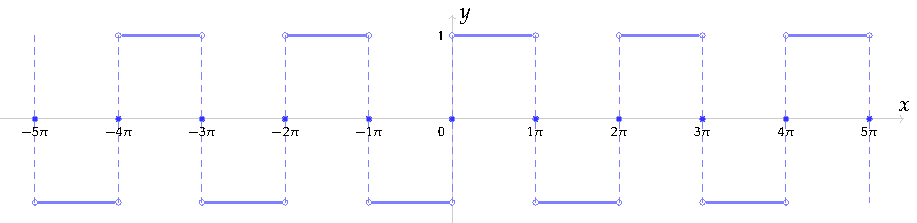
\includegraphics[width=14cm]{image/RecWave.pdf}
        \caption{方波的图像}
    \end{figure}
\end{frame}

\begin{frame}
    \frametitle{方波的傅里叶展开}
    我们如何认识方波?
    \begin{itemize}
        \item 方波可以视为一个随时间变化的函数$f(x)$,有时为$1$,有时为$-1$。
        \item 方波亦可以视为一系列不同频率的正弦函数$\sin\omega x$按比例$F(\omega)$的叠加。
    \end{itemize}

    换言之,我们可以建立这样一种对应关系
    \begin{equation}
        f(x)\leftrightarrow F(\omega)=\frac{4}{\pi\omega},\quad\text{当$\omega$为奇数}
    \end{equation}
    其实,这就是傅里叶变换的核心思想。
\end{frame}

\begin{frame}
    \frametitle{傅里叶变换的核心思想}
    傅里叶变换的核心思想在于,同样一个函数(随时间变化的信号)
    \begin{itemize}
        \item 我们可以在时域$f\,(x)$上描述,即信号随时间如何变化。
        \item 我们可以在频率$F(\omega)$上描述,即信号中各个频率的简谐波的成分有多少。
    \end{itemize}
    傅里叶变换研究的,就是时域函数$f\,(x)$和频域函数$F(\omega)$之间如何转化。

    频域函数$F(\omega)$的实质,就是傅里叶级数中的“叠加系数$b_n$”,但换了一种写法。
\end{frame}

\subsection{傅里叶变换}

\begin{frame}
    \frametitle{傅里叶级数到傅里叶变换}
    然而,要从傅里叶级数正式过渡到傅里叶变换,我们还要克服两个困难
    \begin{enumerate}
        \item 傅里叶级数的有正弦和余弦两套叠加系数,谁将作为频域函数?
        \item 傅里叶级数只能适用于周期函数,那非周期函数如何处理?
    \end{enumerate}
\end{frame}

\begin{frame}
    \frametitle{欧拉公式}

    \begin{theorem}[欧拉公式]
        欧拉公式建立了三角函数与复指数间的联系
        \begin{equation}
            \e^{\i\theta}=\cos\theta+\i\sin\theta
        \end{equation}
    \end{theorem}

    欧拉公式亦可以反过来用,即将三角函数展开为复指数
    \begin{equation}
        \cos\theta=\frac{\e^{\i\theta}+\e^{-\i\theta}}{2}\qquad
        \sin\theta=\frac{\e^{\i\theta}-\e^{-\i\theta}}{2\i}
    \end{equation}
\end{frame}

\begin{frame}
    \frametitle{傅里叶级数的复数形式}
    根据傅里叶级数的展开式
    \begin{equation}
        f(x)
        =a_0+\Sum[n=1][\infty]{\qty[a_n\cos\frac{n\pi}{L}x+b_n\sin\frac{n\pi}{L}x]}
    \end{equation}
    运用欧拉公式
    \begin{equation}
        f(x)=a_0+\Sum[n=1][\infty]{\qty[
                    \frac{a_n}{2}\qty(
                    \e^{\i\frac{n\pi}{L}x}+
                    \e^{-\i\frac{n\pi}{L}x})+
                    \frac{b_n}{2\i}\qty(
                    \e^{\i\frac{n\pi}{L}x}-
                    \e^{-\i\frac{n\pi}{L}x})]}
    \end{equation}
\end{frame}

\begin{frame}
    \frametitle{傅里叶级数的复数形式}
    稍作整理
    \begin{equation}
        f(x)=a_0+\Sum[n=1][\infty]{\qty[
                    \frac{a_n-\i b_n}{2}
                    \e^{\i\frac{n\pi}{L}x}+
                    \frac{a_n+\i b_n}{2}
                    \e^{-\i\frac{n\pi}{L}x}]}
    \end{equation}
    我们期望的形式是
    \begin{equation}
        f(x)=\Sum[k=-\infty][\infty]{c_n\e^{\i\frac{k\pi}{L}x}}\qquad
        c_k=
        \begin{cases}
            \mal{\frac{a_n-\i b_n}{2}},&k>0,~n=+k\\[3mm]
            \mal{a_0},&k=0\\[3mm]
            \mal{\frac{a_n+\i b_n}{2}},&k<0,~n=-k
        \end{cases}
    \end{equation}
\end{frame}

\begin{frame}
    \frametitle{傅里叶级数的复数形式}
    分析系数
    \begin{align}
        a_0&=\frac{1}{2L}\Int[-L][L]{f(t)\dd{t}}\\[6pt]
        \frac{a_n-\i b_n}{2}
        &=\frac{1}{2L}
        \Int[-L][L]{f(t)\qty[\cos\frac{n\pi}{L}t-\i\sin\frac{n\pi}{L}t]\dd{t}}=
        \frac{1}{2L}
        \Int[-L][L]{f(t)\e^{-\i\frac{n\pi}{L}t}\dd{t}}\\[6pt]
        \frac{a_n+\i b_n}{2}
        &=\frac{1}{2L}
        \Int[-L][L]{f(t)\qty[\cos\frac{n\pi}{L}t+\i\sin\frac{n\pi}{L}t]\dd{t}}=
        \frac{1}{2L}
        \Int[-L][L]{f(t)\e^{\i\frac{n\pi}{L}t}\dd{t}}
    \end{align}
\end{frame}

\begin{frame}
    \frametitle{傅里叶级数的复数形式}
    因此,$c_k$的形式是统一的
    \begin{equation}
        c_k=\frac{1}{2L}
        \Int[-L][L]{f(t)\e^{-\i\frac{k\pi}{L}t}\dd{t}}
    \end{equation}
    至此,我们就成功的将傅里叶级数转换为了复数形式。
\end{frame}

\begin{frame}
    \begin{theorem}[傅里叶级数的复数形式]
        设$f(x)$是周期为$2L$的周期函数,即满足$f(x)=f(x+2L)$,且在$[-L,L]$上可积。

        若$f(x)$可以展开为以下形式的傅里叶级数
        \begin{equation}
            f(x)=\Sum[k=-\infty][\infty]{c_k\e^{\i\frac{k\pi}{L}x}}
        \end{equation}
        那系数$c_k$满足
        \begin{gather}
            c_k=\frac{1}{2L}
        \Int[-L][L]{f(t)\e^{-\i\frac{k\pi}{L}t}\dd{t}}
        \end{gather}
    \end{theorem}  
\end{frame}

\begin{frame}
    \frametitle{傅里叶变换的引入}
    \begin{center}
        非周期函数可以视为一个周期$L\to\infty$的周期函数。
    \end{center}
\end{frame}

\begin{frame}
    \frametitle{傅里叶变换的引入}
    \begin{center}
        傅里叶变换的实质,就是傅里叶级数的复数形式在周期$L\to\infty$的极限形态。
    \end{center}
\end{frame}

\begin{frame}
    \frametitle{傅里叶变换的引入}
    取傅里叶变换的复数形式$L\to\infty$的极限
    \begin{equation}
        f(x)=\Lim[L\to\infty]\Sum[k=-\infty][\infty]{c_k\e^{\i\frac{k\pi}{L}x}}
    \end{equation}
    引入代换变量
    \begin{equation}
        \omega=\frac{k\pi}{L}\qquad
        \delt{\omega}=\frac{\pi}{L}
    \end{equation}
    这里$\omega,\delt{\omega}$的意义是清楚的,$\omega$代表$k$时的频率,$\delt{\omega}$代表频率间隔。
\end{frame}

\begin{frame}
    \frametitle{傅里叶变换的引入}
    运用代换变量,$f(x)$的展开式可以改写为
    \begin{equation}
        f(x)=\Lim[L\to\infty]\Sum[k=-\infty][\infty]c_k\e^{\i\omega x}=\Lim[L\to\infty]\Sum[k=-\infty][\infty]\frac{Lc_k}{\pi}\e^{\i\omega x}\delt{\omega}
    \end{equation}
    而和式的极限,就是积分(当$L\to\infty$时有$\delt\omega\to 0$成立)
    \begin{equation}
        f(x)=\frac{1}{\pi}\Int[-\infty][\infty]\Lim[L\to\infty](Lc_k)\e^{\i\omega x}\dd{\omega}
    \end{equation}
\end{frame}

\begin{frame}
    \frametitle{傅里叶变换的引入}
    而$(Lc_k)$的在$L\to\infty$的极限很容易计算
    \begin{equation}
        \Lim[L\to\infty](Lc_k)=\Lim[L\to\infty]\qty(\frac{L}{2L}
        \Int[-L][L]{f(t)\e^{-\i\frac{k\pi}{L}t}\dd{t}})=\frac{1}{2}\Int[-\infty][\infty]f(t)\e^{-\i\omega t}\dd{t}
    \end{equation}
    如果我们记
    \begin{equation}
        F(\omega)=\frac{2}{\sqrt{2\pi}}\Lim[L\to\infty](Lc_k)=\frac{1}{\sqrt{2\pi}}\Int[-\infty][\infty]f(t)\e^{-\i\omega t}\dd{t}
    \end{equation}
    就有
    \begin{equation}
        f(x)=\frac{1}{\pi}\Int[-\infty][\infty]\Lim[L\to\infty](Lc_k)\e^{\i\omega x}\dd{\omega}=\frac{1}{\sqrt{2\pi}}\Int[-\infty][\infty]F(\omega)\e^{\i\omega x}\dd{\omega}
    \end{equation}
\end{frame}

\begin{frame}
    \begin{theorem}[傅里叶变换]
        设$f(x)$是定义在$(-\infty~~,\infty)$上的函数,并且在$(-\infty~~,\infty)$上绝对可积。

        那么定义$F(\omega)$为函数$f(x)$的傅里叶变换
        \begin{equation}
            F(\omega)=\frac{1}{\sqrt{2\pi}}\Int[-\infty][\infty]f(x)\e^{-\i\omega x}\dd{x}=\F{f(x)}
        \end{equation}
        其中$\e^{-\i\omega x}$称为傅里叶变换的核。而$f(x)$则称为函数$F(\omega)$的傅里叶逆变换
        \begin{equation}
            f(x)=\frac{1}{\sqrt{2\pi}}\Int[-\infty][\infty]F(\omega)\e^{\i\omega x}\dd{\omega}=\F*{F(\omega)}
        \end{equation}
        以上,将$F(\omega)$称为像函数,而将$f(x)$称为原函数。
    \end{theorem}  
\end{frame}

\begin{frame}
    \frametitle{傅里叶变换的一个重要性质}

    傅里叶变换有许多性质,这里我们要证明一个对今天的内容尤为重要的性质。

    \begin{theorem}[傅里叶变换的相似性质]
        设原函数$f(x)$,以及像函数$\F{f(x)}=F(\omega)$,对于任意实数$\lambda$,有
        \begin{equation}
            \F{f(\lambda x)}=\frac{1}{\abs{\lambda}}F\qty(\frac{\omega}{\lambda})
        \end{equation}
    \end{theorem}
\end{frame}

\begin{frame}
    \frametitle{傅里叶变换的一个重要性质}
    证明是容易的,根据傅里叶变换的定义
    \begin{equation}
        \F{f(\lambda x)}=\frac{1}{\sqrt{2\pi}}\Int[-\infty][\infty]{f(\lambda x)\e^{-\i\omega x}\dx}
    \end{equation}
    上式中作代换$\xi=\lambda x$,注意到$\dx=\dd{\xi}/\lambda$
    \begin{equation}
        \F{f(\lambda x)}=\frac{1}{\abs{\lambda}}\frac{1}{\sqrt{2\pi}}\Int[-\infty][\infty]f(\xi)\e^{-\i\frac{\omega}{\lambda}\xi}\dd{\xi}=\frac{1}{\abs{\lambda}}F\qty(\frac{\omega}{\lambda})
    \end{equation}
    上式出现$\abs{\lambda}$的原因是当$\lambda<0$时代换后积分限变为$(\infty,-\infty)$,而此时$\abs{\lambda}=-\lambda$。
\end{frame}

\begin{frame}
    \frametitle{傅里叶变换的一个重要性质}
    傅里叶变换的相似性质指出
    \begin{itemize}
        \item 时域上的压缩,在频域上表现为等比例的横向拉伸和纵向压缩。
        \item 时域和频域无法同时被压缩。
    \end{itemize}
\end{frame}
\section{傅里叶变换与不确定性原理}

\begin{frame}
    \frametitle{位置?动量?}
    我们知道,在量子力学中,粒子的位置服从波函数的概率分布,实际上,粒子的动量亦服从概率分布。因为微观粒子并没有确定的轨道,即没有确定的位置和动量。

    现在的问题是,动量服从何种概率分布呢?
\end{frame}

\begin{frame}
    \frametitle{位置和动量间的傅里叶关系}
    实际上,在量子力学中
    \begin{center}
        动量,是位置的傅里叶变换。
    \end{center}
    % 更确切的说,动量遵循的概率分布$\phi(\vb*{p})$是波函数$\psi(\vb*{r})$的傅里叶变换。

    为什么动量$\vb*{p}$和位置$\vb*{r}$两个看似毫无关系的物理量,会通过傅里叶变换相联系?
\end{frame}

\begin{frame}
    \frametitle{位置和动量间的傅里叶关系}
    波函数$\psi(\vb*{r})$的傅里叶变换直接给出的,姑且记作$\phi_0(\vb*{k})$,描述的是$\psi(\vb*{r})$中各个角波矢$\vb*{k}$的平面简谐波的出现概率,考虑到傅里叶变换是在三维空间中进行的
    \begin{equation}
        \phi_0(\vb*{k})=\frac{1}{(2\pi)^{3/2}}\Itnt\psi(\vb*{r})\exp(-\i\vb*{k}\cdot\vb*{r})\dd^3x
    \end{equation}
    相应的逆变换为
    \begin{equation}
        \psi(\vb*{r})=\frac{1}{(2\pi)^{3/2}}\Itnt\phi_0(\vb*{k})\exp(\i\vb*{k}\cdot\vb*{r})\dd^3k
    \end{equation}
    类比:时域--频域,坐标空间--波矢空间。
\end{frame}

\begin{frame}
    \frametitle{位置和动量间的傅里叶关系}
    根据德布罗意关系式,动量和角波矢间具有简单关系
    \begin{equation}
        \vb*{p}=\hbar\vb*{k}
    \end{equation}
    这意味着,傅里叶变换的像空间,既可以使用波矢空间,也可以使用动量空间。
\end{frame}

\begin{frame}
    这样,通过变量代换,就可以由$\vb*{k}$的概率幅得到$\vb*{p}$的概率幅
    \begin{equation}
        \phi(\vb*{p})=
        \phi_0(\vb*{p}/\hbar)=
        \frac{1}{(2\pi)^{3/2}}\Itnt\psi(\vb*{r})
        \exp(-\i\vb*{p}\cdot\vb*{r}/\hbar)\dd^3x
    \end{equation}
    由于$\dd^3k=\dd^3p/\hbar^3$,逆变换可以改写为
    \begin{equation}
        \psi(\vb*{r})=\frac{1}{(2\pi)^{3/2}}\frac{1}{\hbar^3}\Itnt\phi(\vb*{p})\exp(\i\vb*{p}\cdot\vb*{r}/\hbar)\dd^3p
    \end{equation}
    这里$1/\hbar^3$位于逆变换,但可以将其拆分为两个$1/\hbar^{3/2}$并均等的置于变换和逆变换。
\end{frame}

\begin{frame}
    \begin{theorem}[波函数的傅里叶变换]
        \setlength{\parskip}{0pt}
        记波函数$\psi(\vb*{r})$的傅里叶变换为$\phi(\vb*{p})$
        \begin{equation}
            \phi(\vb*{p})=\frac{1}{(2\pi\hbar)^{3/2}}\Itnt\psi(\vb*{r})\exp(-\i\vb*{p}\cdot\vb*{r}/\hbar)\dd^3x
        \end{equation}
        记相应逆变换为
        \begin{equation}
            \psi(\vb*{r})=\frac{1}{(2\pi\hbar)^{3/2}}\Itnt\phi(\vb*{p})\exp(\i\vb*{p}\cdot\vb*{r}/\hbar)\dd^3p
        \end{equation}
        那么,波函数$\psi(\vb*{r})$和波函数的傅里叶变换$\phi(\vb*{p})$将具有以下意义
        \begin{itemize}
            \item $\abs{\psi(\vb*{r})}^2$表示了粒子的位矢为$\vb*{r}$的概率密度。
            \item $\abs{\phi(\vb*{p})}^2$表示了粒子的动量为$\vb*{p}$的概率密度。
        \end{itemize}
    \end{theorem}
\end{frame}

\begin{frame}
    \frametitle{位置和动量间的傅里叶关系}
    动量和位置间的傅里叶关系,本质上,是德布罗意关系式$\vb*{p}=\hbar\vb*{k}$的结果
\end{frame}

\begin{frame}
    \frametitle{不确定性原理}
    不确定性原理:经典粒子中轨道的想法对于微观粒子究竟在多大程度上适用?

    \begin{itemize}
        \item 粒子的位置服从$|\psi(\vb*{r})|^2$的分布
        \item 粒子的动量服从$|\phi(\vb*{p})|^2$的分布
    \end{itemize}
    因此,只能说,粒子的位置和动量有较大概率处于某一范围内,无法给出确切值。
\end{frame}

\begin{frame}
    \begin{columns}[t] 
        \begin{column}{7cm} 
            \begin{figure}
                \includegraphics[width=6cm]{build/Section3_01.fig.pdf}
                \caption{位矢的概率密度分布}
            \end{figure}
        \end{column}
        \begin{column}{7cm} 
            \begin{figure}
                \includegraphics[width=6cm]{build/Section3_02.fig.pdf}
                \caption{动量的概率密度分布}
            \end{figure}
        \end{column}
    \end{columns}
\end{frame}

\begin{frame}
    \frametitle{不确定性原理}
    那么能否同时尽可能准确的测定位置和动量,得到比较准确的轨道?

    遗憾的是,这也是无法完成的。
\end{frame}

\begin{frame}
    \frametitle{不确定性原理}
    动量的概率幅$\phi(\vb*{p})$是位置的概率幅$\psi(\vb*{r})$的傅里叶变换,而相似性质指出
    \begin{equation}
        \F{\sqrt{\lambda}\cdot\psi(\lambda\vb*{r})}=\frac{1}{\sqrt{\lambda}}\cdot\phi\qty(\frac{\vb*{p}}{\lambda})
    \end{equation}
    若记$\delt{x},\delt{p}$为不确定度,则
    \begin{equation}
        \delt{x}\cdot\delt{p}=\text{定值}
    \end{equation}
    由此可见,位置的不确定性$\delt{x}$和动量的不确定性$\delt{p}$将相互制约
    \begin{itemize}
        \item 确定位置($\delt{x}$很小)将导致动量的不确定($\delt{p}$很大)。
        \item 确定动量($\delt{p}$很小)将导致位置的不确定($\delt{x}$很大)。
    \end{itemize}
\end{frame}

\begin{frame}
    \frametitle{不确定性原理}
    \begin{theorem}[不确定原理]
        不确定性关系指出,微观粒子的位置和动量的不确定性是相互制约的
        \begin{equation}
            \delt{x}\cdot\delt{p}\geq\frac{\hbar}{2}
        \end{equation}
    \end{theorem}
\end{frame}

\begin{frame}
    \frametitle{不确定性原理}
    \begin{itemize}
        \item 不确定性原理告诉我们,同时尽可能准确的测出微观粒子的位置和动量的努力存在一个不可逾越,无关测量本身,由量子力学基本原理所决定的物理极限。
        \item 不确定性原理的本质是,由于波粒二象性和德布罗意关系式,微观粒子的位置和动量间存在傅里叶关系,而相似性质表明原函数和像函数不能同时被压缩。
    \end{itemize}
\end{frame}

\section{Q \& A}

\begin{frame}
    \frametitle{Q \& A}
\end{frame}

\end{document}